\chapter{MAGIC-UNet: the paper and our copy}\label{ch:magic}

\section{The paper}

N. R. Reed, D. Bhutto, M. J. Turner, D. M. Daly, S. M. Oliver, J. Tang, K. S. Olsson, N. Langellier, M. J. H. Ku,
M. S. Rosen and R. L. Walsworth, ``Machine learning for improved current-density reconstruction from two-dimensional
vector magnetic images'', \emph{Physical Review Applied} \textbf{23}, 034035 (2025), doi:10.1103/PhysRevApplied.23.034035.
The preprint is arXiv 2407.14553 (2024). The network is a U-Net, and the authors call it MAGIC-UNet (Magnetic Inverse
Calculation UNet).

\begin{keyidea}[How to read the first half of this chapter]
Everything up to Section~\ref{sec:magic_sources} is taken from the published paper, and each statement names the section,
table or figure it comes from, so you can check it. Where the paper is silent, the text says so. Our own calculations are
marked \emph{ours}. Older notes in this repository cite a ``Supplement D''. The published version has no supplement. Its
recipe is in Sec.~V~A, Tables IV and V, and Appendix~A, and its noise analysis is in Appendix~B. Cite those.
\end{keyidea}

\section{The problem they set out to solve}

A QDM measures the vector field $(B_x, B_y, B_z)$ in a plane some distance above a sample. The wanted output is the
planar current density $(J_x, J_y)$ that made it (Sec.~II). The standard tool is the \emph{Fourier method}: invert the
Biot--Savart law in Fourier space. The paper's introduction names its two weak spots (Sec.~I): noise at high spatial
frequency, and a standoff larger than the size of the current features. The workaround is to average many repeated
measurements, which is slow and lets drift creep in.

Why both weak spots are the same problem: for a thin current sheet a distance $z$ below the sensor, every Fourier
component of the field is the matching component of the current times a fixed factor:
\begin{equation}
\hat B(\bm k, z) \;\propto\; \frac{\mu_0}{2}\, e^{-kz}\, \hat J(\bm k), \qquad k = |\bm k|.
\label{eq:magic_decay}
\end{equation}
The paper does not print this equation. For the Fourier transformations it uses, it cites its refs.~[30,~59] (Roth
2023; Broadway et al.\ 2020) in Sec.~V~C. Its ref.~[37] (Roth, Sepulveda and Wikswo 1989) is cited where Sec.~I says the
Fourier method fails on noisy data. Inverting means multiplying by $e^{+kz}$, so noise at large $k$ is amplified
exponentially.

\begin{keyidea}[How bad the amplification is (ours, from Eq.~\ref{eq:magic_decay})]
At the finest scale an image can hold, $k = \pi/\Delta$ for pixel size $\Delta$, the gain is $e^{\pi z/\Delta}$.
\begin{center}
\small
\begin{tabular}{lcccc}
\toprule
Case & $z$ & $\Delta$ & $z/\Delta$ & $e^{\pi z/\Delta}$ \\
\midrule
Paper, main model & 50\um & 31\um & 1.6 & $1.5\times10^{2}$ \\
Paper, large-standoff model & 500\um & 31\um & 16 & $7\times10^{21}$ \\
Ours, run 2 & 3\um & 0.2\um & 15 & $3\times10^{20}$ \\
Ours, 10\um\ runs & 10\um & 0.7\um & 14 & $3\times10^{19}$ \\
\bottomrule
\end{tabular}
\end{center}
Measured in pixels, our problem is like the paper's \emph{large-standoff} case, not its main one. Keep this in mind for
Section~\ref{sec:magic_limits}.
\end{keyidea}

\section{The question this paper settles: is the network told the standoff?}\label{sec:magic_standoff}

No. Three places in the paper say so:
\begin{enumerate}
\item \textbf{Sec.~III, second paragraph.} The synthetic validation images each have a standoff drawn from a normal
distribution with mean 50\um\ and standard deviation 10\um, chosen to mimic the spread of a real experiment. The Fourier
method is given the exact standoff of each image. MAGIC-UNet is not, and the authors call that a practical feature for
experiments.
\item \textbf{Table V.} The standoff is $50\pm10$\um\ for both wire classes in the training and validation data, and
$500\pm50$\um\ for the large-standoff model.
\item \textbf{Sec.~V~C.} The same distribution, mean 50\um\ and standard deviation 10\um, is described as approximating
the real separation between the NV layer and the current traces in their circuit board.
\end{enumerate}

\begin{careful}[What this means for our claims]
``A network that reconstructs the current without being told the standoff, inside a band of about $\pm20\%$'' is the
paper's result, not ours. Do not present it as new. The paper does \emph{not}:
\begin{itemize}
\item use one network across very different standoffs. The 500\um\ case is a \emph{separate} network trained at
$500\pm50$\um\ (Sec.~III~C, Table~V);
\item output a standoff, or an uncertainty;
\item give the field at another height. It stops at the current.
\end{itemize}
Also note the comparison in the paper is generous to the baseline. The Fourier method gets the exact standoff and a
tuned filter (Section~\ref{sec:magic_fourier}); MAGIC-UNet gets neither.
\end{careful}

The standoffs actually tested sit inside or near the training band: 40$\pm$5\um\ for the noise sweep (Fig.~3), 65\um\ and
36\um\ for the experimental images of Fig.~4, 45\um\ for the Hilbert-curve images of Fig.~5, and about 500\um\ for the
large-standoff network (Fig.~6). The experimental standoffs ranged over 36--65\um\ and 486--650\um\ (Sec.~V~B).

\section{Training data (Sec.~V~A, Appendix~A, Table~V)}

The current comes first, the field second. Random wire shapes are drawn, then COMSOL and MATLAB finite-element runs give
the current density that flows when a voltage is put across the conductor, so the current bends around corners
realistically (Sec.~V~A, Fig.~8). The field is then computed from that current with the Biot--Savart law written as a
Fourier transform, with no noise at this stage (Appendix~A).

\begin{center}
\small
\begin{tabularx}{\textwidth}{>{\raggedright\arraybackslash}p{3.4cm}>{\raggedright\arraybackslash}X>{\raggedright\arraybackslash}X}
\toprule
Parameter (Table V) & Class I & Class II \\
\midrule
Wires & Curves through 2--21 random points (cropped); can loop and short when they cross & Thin right-angle segments,
thin segments at any angle, thick straight wires \\
Independent wires & 1 & 1, 2 or 3 (closely spaced planes) \\
Field of view & 2\,mm & 2\,mm \\
Standoff & $50\pm10$\um\ ($500\pm50$\um\ large standoff) & $50\pm10$\um\ ($500\pm50$\um\ large standoff) \\
Current layer & 14\um\ thick & 14\um\ thick \\
Wire width & 16--160\um\ (50\%), 160--320\um\ (50\%) & 9--30\um\ (67\%), 97--156\um\ (33\%) \\
Current & 15.5--311\,mA & 1.95--170\,mA \\
\bottomrule
\end{tabularx}
\end{center}

\begin{itemize}
\item \textbf{Size.} 153{,}600 training pairs and 4{,}096 pairs for validation and testing (Sec.~V~A). Images are
$64\times64$, so a 2\,mm view gives pixels of about 31\um, the same as their binned experimental images (Sec.~V~B).
\item \textbf{Augmentation.} A $90^\circ$ rotation, a horizontal flip and a vertical flip, each applied with probability
1/2, giving eight variants (Appendix~A).
\item \textbf{Fields from outside.} About 2\% of the training images have wires only outside the field of view, so the
network learns what fields from outside look like (Appendix~A).
\item \textbf{Scaling.} Each input image $i$ is divided by its own scalar $\alpha_i$, and its target current by the same
$\alpha_i$. All targets are also multiplied by one global $\beta\approx10^{8}$, which is divided out after prediction
(Appendix~A). The paper does \emph{not} say how $\alpha_i$ is computed.
\item \textbf{Noise.} Fresh additive Gaussian noise is drawn between every epoch (Appendix~A). The authors chose it after
measuring their real noise (Appendix~B, Section~\ref{sec:magic_limits}). The training noise level is \emph{not} stated.
\end{itemize}

\section{The network (Sec.~II, Fig.~1)}

\begin{figure}[H]
\centering
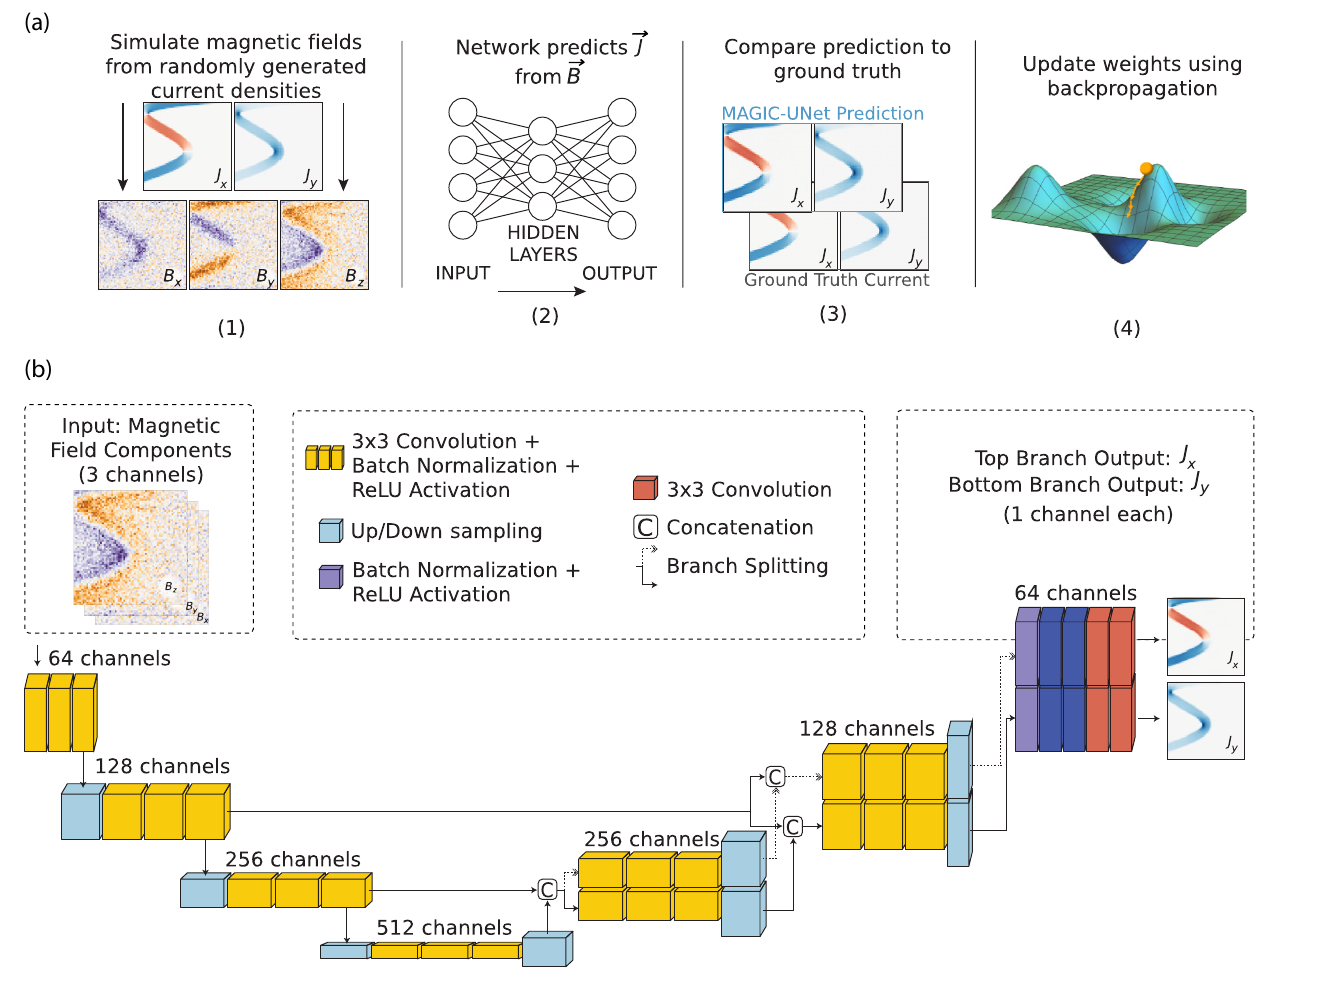
\includegraphics[width=\textwidth]{reed_fig1}
\caption{(a) The training loop: simulate fields from random currents, predict, compare by mean squared error, update by
backpropagation. (b) MAGIC-UNet. Yellow: $3\times3$ conv, BatchNorm, ReLU. Light blue: down- or upsampling. Purple:
BatchNorm and ReLU. Red: $3\times3$ conv. The two output branches, one for $J_x$ and one for $J_y$, never interact.
\emph{Source:} Reed et al., Phys.\ Rev.\ Applied \textbf{23}, 034035 (2025), Fig.~1, CC BY 4.0; cropped, otherwise
unchanged.}
\label{fig:reed_fig1}
\end{figure}

What Sec.~II says, step by step:
\begin{enumerate}
\item \textbf{Encoder.} At each level, a padded $3\times3$ conv, BatchNorm and ReLU, three times, then $2\times2$
average pooling. The text says ``a stride of 1''; see Section~\ref{sec:magic_sources} for why we use 2. The resolution
halves and the channels double at each of three steps: 64, 128, 256, then 512 at the bottom.
\item \textbf{Why average pooling.} Max pooling keeps only the strongest pixel. Every detail of the field matters here, so
they average.
\item \textbf{Skips.} Encoder outputs are concatenated with the decoder at the same resolution. The first (64-channel)
skip is left out because it did not help.
\item \textbf{Two decoders.} After the bottom, the network splits. Each branch upsamples by $2\times2$ with a convolution,
concatenates the skip, and applies conv, BatchNorm and ReLU three times. One branch outputs $J_x$, the other $J_y$. Read
literally that is four convolutions per decoder level; Section~\ref{sec:magic_sources} explains why the released model
has three.
\end{enumerate}

\section{Training (Table~IV)}

\begin{center}
\small
\begin{tabular}{lllllll}
\toprule
Optimiser & Learning rate & Epochs & Batch & Loss & Library & GPU \\
\midrule
RMSprop & $10^{-4}$ & 50 & 32 & MSE & TensorFlow 2.10.0 & RTX A6000, 48\,GB \\
\bottomrule
\end{tabular}
\end{center}

Training took 11 hours (Table~IV). Why MSE: it is the maximum-likelihood loss for Gaussian noise, which is what they
measured in real data (Sec.~III~A).

\section{The baseline they beat: a tuned Fourier method (Sec.~V~C)}\label{sec:magic_fourier}

The authors did not compare against a naive inversion. They tuned it:
\begin{itemize}
\item they use $B_x$ and $B_y$ rather than $B_z$, which is more robust (following Broadway et al.\ [59]);
\item they apply a Gaussian filter against aliasing and the finite Fourier bandwidth, and a Hann window against noise
(the Hann window following their ref.~[37]);
\item they search the window and filter strengths in three dimensions, for several standoffs, to maximise SSIM on
synthetic data;
\item and they give it the exact standoff of each image (Sec.~III).
\end{itemize}

\section{How they measure noise and quality (Sec.~III, Appendix~C)}

\textbf{Noise level.} The noise is set relative to the strongest field in the image:
\begin{equation}
\sigma_n = \frac{\sigma}{\max_{\text{pixels}} |\bm B|}.
\label{eq:magic_sigma_n}
\end{equation}
That is, Gaussian noise of standard deviation $\sigma = \sigma_n \max|\bm B|$ is added to the field.
So $\sigma_n = 0.2$ means a noise standard deviation of one fifth of the peak field. The paper relates $\sigma_n = 0.5$
to an input SNR of about 2, and $\sigma_n = 1$ to SNR about 1.

\textbf{SNR of real images} (Appendix~C). Along a strong wire segment, take the peak field on each line cut across it and
average those peaks. Divide by the standard deviation of the pixels in a quiet region.

\textbf{Quality.} SSIM (structural similarity) is the main score, with the rule of thumb they quote: 0.95--0.99 is close
to perfect, 0.88--0.95 is fair, below 0.88 is poor, below 0.50 is bad (Sec.~III, refs.~[52,~53]). They also report RMSE
and PSNR.

\section{What they found}

\begin{figure}[H]
\centering
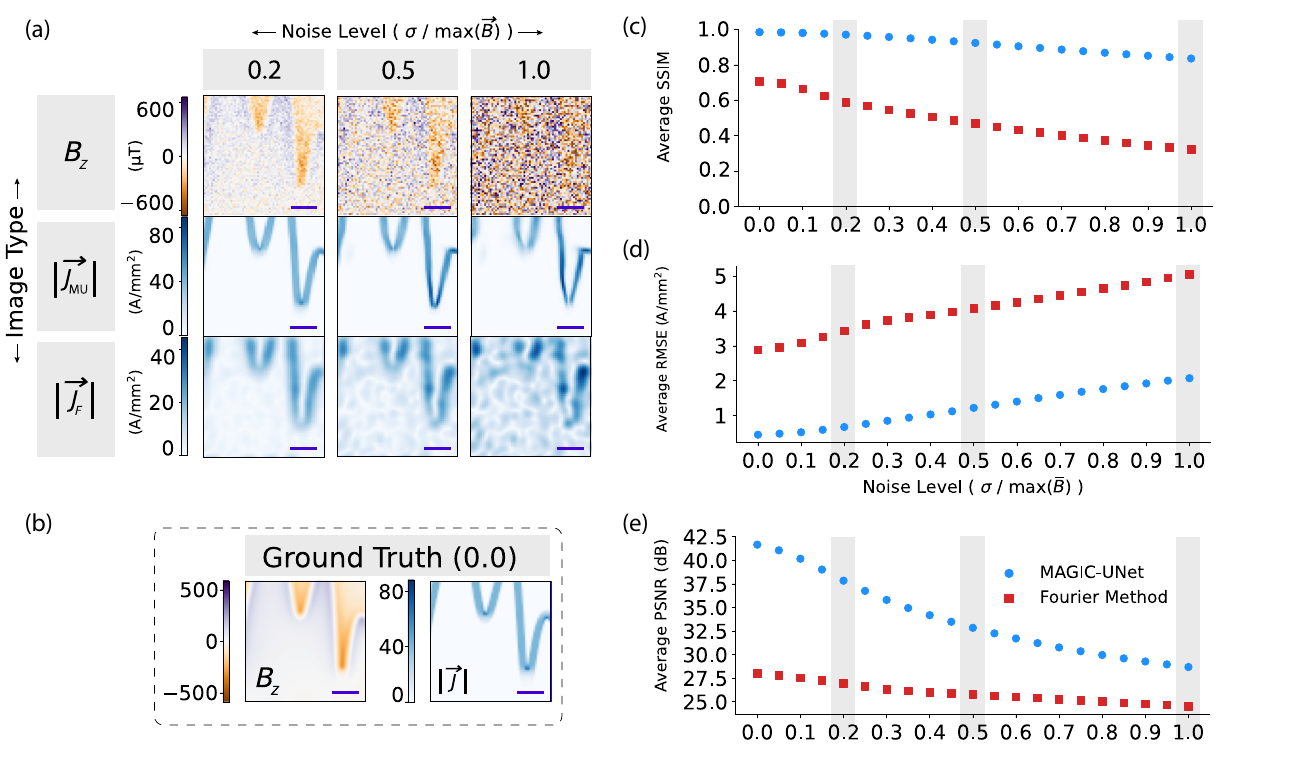
\includegraphics[width=\textwidth]{reed_fig3}
\caption{The noise sweep, at standoff $40\pm5$\um. (a) $B_z$ at $\sigma_n = 0.2$, 0.5 and 1.0, with the current magnitude
from MAGIC-UNet (middle row) and from the Fourier method (bottom row). (b) The truth. (c)--(e) Average SSIM, RMSE and PSNR
against $\sigma_n$: MAGIC-UNet blue circles, Fourier method red squares. \emph{Source:} Reed et al., Phys.\ Rev.\ Applied
\textbf{23}, 034035 (2025), Fig.~3, CC BY 4.0; cropped, otherwise unchanged.}
\label{fig:reed_fig3}
\end{figure}

\begin{center}
\small
\begin{tabular}{lcc}
\toprule
Score, from $\sigma_n = 0$ to $\sigma_n = 1$ (Fig.~3, Sec.~III~A) & MAGIC-UNet & Fourier method \\
\midrule
SSIM & 0.99 $\to$ 0.84 & 0.71 $\to$ 0.32 \\
PSNR & 41.7 $\to$ 28.7\,dB & 28.0 $\to$ 24.5\,dB \\
RMSE & \multicolumn{2}{c}{Fourier about 3--4 times larger at every level} \\
\bottomrule
\end{tabular}
\end{center}

\begin{itemize}
\item MAGIC-UNet stays above SSIM 0.95 up to $\sigma_n = 0.35$ (SNR above 2.8), and above 0.88 for $\sigma_n$ between
0.40 and 0.70 (Sec.~III~A).
\item Sec.~IV quotes a different comparison, for the $64\times64$ network at 50\um\ (Fig.~3 is at $40\pm5$\um): the
RMSE is about 10 times lower than the Fourier method's without noise, and about 2.5 times lower at
SNR 1. MAGIC-UNet at $\sigma_n = 1$ beats the Fourier method at $\sigma_n = 0$ on all three scores (Sec.~IV). Their
headline: SNR-1 inputs to MAGIC-UNet were more accurate than SNR-20 inputs to the Fourier method, which means data
collected 400 times faster.
\item By wire class (Table I), MAGIC-UNet SSIM is 0.895--0.962, against 0.356--0.519 for the Fourier method. $J_x$ and
$J_y$ are equally good (within 1\%).
\item Out of distribution: COMSOL-made straight and curved wires reach SSIM 0.962 at $\sigma_n = 0.5$. Branching wires of
uneven width reach only 0.88, so the network ``has not learned a fully general version of the inversion'' (Sec.~III~A).
\item Larger images (Sec.~III~B, Table~III). A separate $256\times256$ network beats the $64\times64$ one at high noise
on synthetic data (SSIM 0.923 against 0.836 at $\sigma_n = 1$), but is worse on noisy experimental data. Tiling with the
$64\times64$ network works well: overlapping $64\times64$ tiles, overlaps divided equally between neighbours,
duplicates discarded (Fig.~5c). It works even when a tile covers a field of view four times smaller than the training
images.
\end{itemize}

\section{Their limits, from the paper}\label{sec:magic_limits}

\subsection{Correlated noise in real data (Appendix~B)}

\begin{figure}[H]
\centering
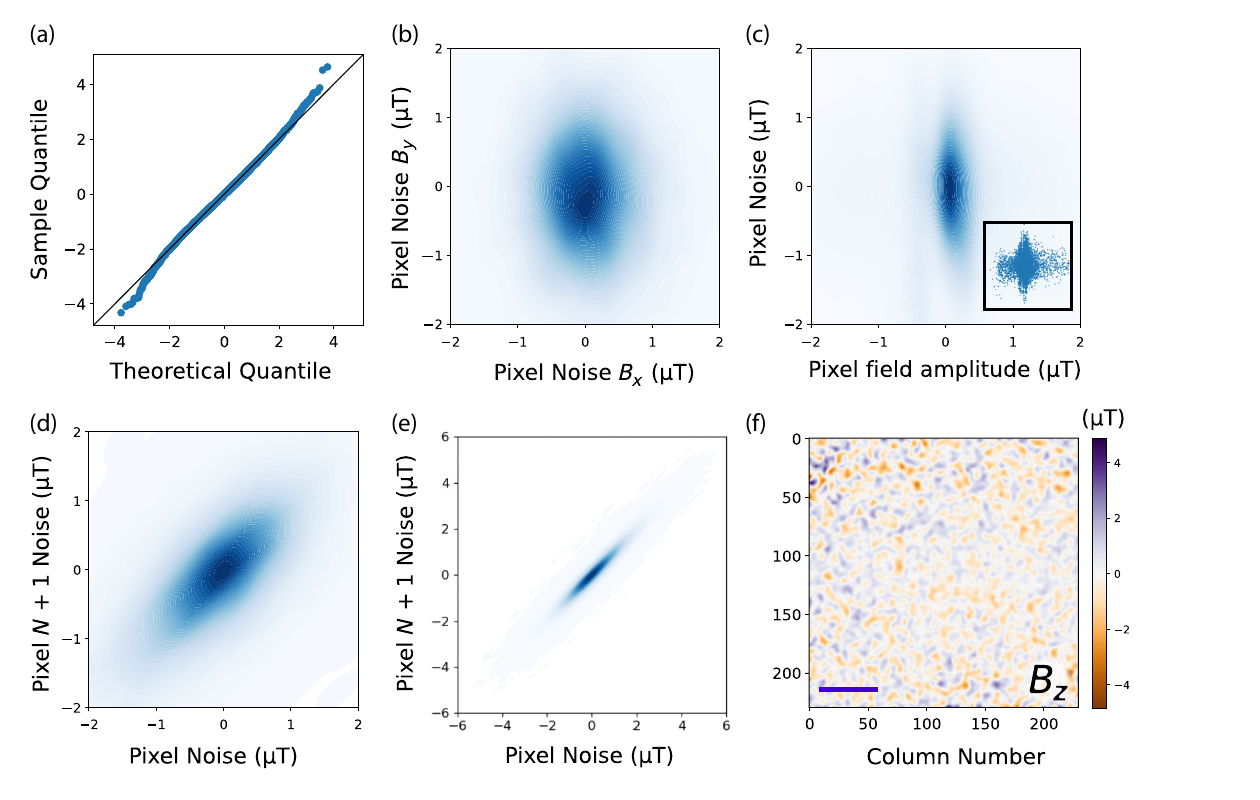
\includegraphics[width=\textwidth]{reed_fig10}
\caption{Noise in real QDM images, from low-SNR minus high-SNR maps of the same view. (a) Quantile plot: close to
Gaussian. (b) $B_x$ noise against $B_y$ noise: uncorrelated. (c) Noise against field amplitude: additive, not growing
with the field. (d), (e) Each pixel's noise against its neighbour's, at $64\times64$ and $230\times230$: strongly
correlated. (f) A $B_z$ noise map with blobs 5--10 pixels wide. \emph{Source:} Reed et al., Phys.\ Rev.\ Applied
\textbf{23}, 034035 (2025), Fig.~10, CC BY 4.0; cropped, otherwise unchanged.}
\label{fig:reed_fig10}
\end{figure}

Real QDM noise is Gaussian, additive and uncorrelated between components, so white Gaussian training noise is a
reasonable model, except in one respect: neighbouring pixels are correlated, $R^2 = 0.60$ at $64\times64$ and
$R^2 = 0.95$ at $230\times230$. The authors blame the ODMR fitting step. MAGIC-UNet shows more artefacts on real images
than on synthetic ones at the same $\sigma_n$ (Sec.~III, Fig.~4). Their two suggested fixes: reduce the correlation in the
measurement, or put correlation into the training noise. Our \code{--noise-corr-um} ablation is the second fix.

\subsection{Several current planes (Table~II)}

SSIM falls from 0.966 with one plane to 0.902 with two and 0.842 with three closely spaced planes. The Fourier method
stays near 0.41 throughout.

\subsection{Large standoff (Sec.~III~C, Fig.~6)}

\begin{figure}[H]
\centering
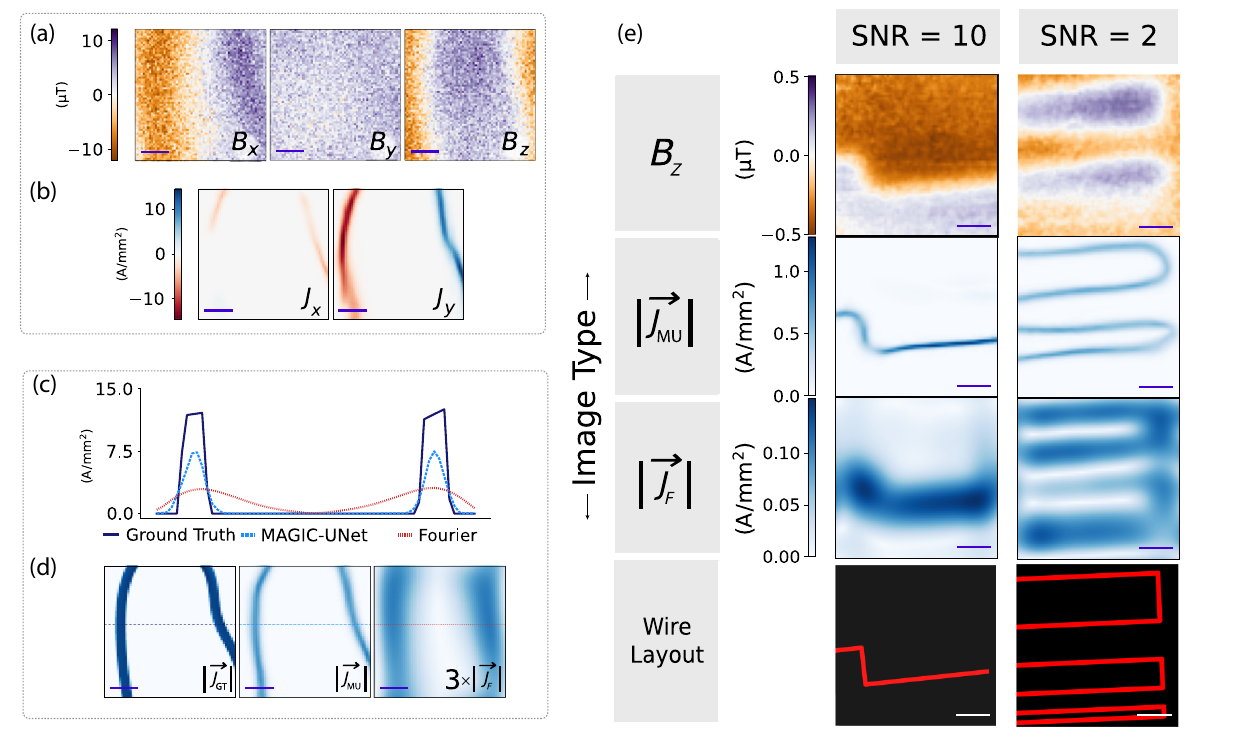
\includegraphics[width=\textwidth]{reed_fig6}
\caption{The large-standoff network, trained at $500\pm50$\um. (a) Synthetic field at 500\um, $\sigma_n = 0.2$. (b)
MAGIC-UNet's $J_x$, $J_y$. (c) A line cut: truth (dark), MAGIC-UNet (blue), Fourier method (red). (d) Current
magnitude: truth, MAGIC-UNet, and three times the Fourier method. (e) Real QDM data at about 500\um, at SNR 10 and 2.
\emph{Source:} Reed et al., Phys.\ Rev.\ Applied \textbf{23}, 034035 (2025), Fig.~6, CC BY 4.0; cropped, otherwise
unchanged.}
\label{fig:reed_fig6}
\end{figure}

A separate $64\times64$ network was trained at $500\pm50$\um, about 5 to 10 times the size of the current features
(Sec.~III~C). There, the paper reports that \emph{both} methods do too poorly for its quantitative scores to mean
anything, and gives no SSIM. Qualitatively MAGIC-UNet is better: wires of roughly the right width in roughly the right
place, where the Fourier method gives a blur. But it has more artefacts than at 50\um, rounded corners, and in the line
cut of Fig.~6(c) its peak current is clearly below the truth.

\begin{careful}[Which of their regimes our tiles are in (ours)]
The field of view is 2\,mm in both of the paper's models (Table~V). So its main model's tile is $2000/50 = 40$
standoffs wide, and its large-standoff model's tile is $2000/500 = 4$. Our run 2 tile is $12.8/3 \approx 4.3$ standoffs
wide; our 10\um\ runs are at $44.8/10 \approx 4.5$. By the pixel count of the earlier table too, $z/\Delta \approx 15$ for
us and 16 for their large-standoff model.

The paper itself defines its large-standoff case by a third ratio, standoff over feature size, ``about 5 to 10 times''
(Sec.~III~C). Our simulator draws wire widths of 1.6--3.2\um\ (\code{simulate_fields.py}), so run 2 is at
$3/3.2$ to $3/1.6$, about 1--2 times, which is nearer their 50\um\ model (50\um\ over widths of 9--320\um, Table~V).
Our 10\um\ runs are at about 3--6 times, near their large-standoff case.

So on tile size and pixels, the paper \emph{did} test our regime, and found its network qualitatively better than
Fourier but not good enough to score. Most of the field in each tile comes from wires outside it. Our results in Chapter~\ref{ch:magic_results} are
measurements in that harder regime, not repeats of the 50\um\ result.
\end{careful}

\section{Four sources, and which one we follow}\label{sec:magic_sources}

That is the paper. The exact architecture needed some detective work, because the sources disagree.
\begin{enumerate}
\item \textbf{The paper} gives the design (Sec.~II, Fig.~1) and the training recipe (Table~IV, Appendix~A).
\item \textbf{The released trained model} (Harvard Dataverse, doi:10.7910/DVN/SD6PVP, the paper's ref.~[61]) contains the
full layer graph. It settles details the text leaves open: pooling stride 2 (the text of Sec.~II says 1), nearest-neighbour
upsampling followed by a $3\times3$ conv without BatchNorm, the order of concatenation, and the initialisation. It also
differs from the text on the decoder: Sec.~II describes an upsampling convolution, then three conv--BatchNorm--ReLU
blocks after the concatenation (four convolutions); the released model has the upsampling conv, BatchNorm and ReLU, then
two blocks (three convolutions). Fig.~1b draws the last, 64-channel level the released way (purple BatchNorm--ReLU, two
blocks, two red convs) and the 256- and 128-channel levels with three yellow blocks. Where they disagree we follow the
released model, because its parameters match the published checkpoint. It has 15,505,194 trainable parameters.
\item \textbf{The released training code} does \emph{not} match either: a different U-Net with tanh and no BatchNorm, a
learning rate of $10^{-5}$, 25 epochs and batch 16. It looks like an older version, so we ignored it.
\item \textbf{Our adaptations}, listed below, each labelled as ours.
\end{enumerate}
So the architecture comes from the released model, and the training recipe from the paper.

\section{Our code}

Each decoder level upsamples, applies a $3\times3$ conv, joins the encoder's skip, then normalises and applies two more
blocks:

\begin{code*}{magic_unet.py}
    def forward(self, x, skip=None):
        x = self.conv(self.up(x))
        if self.skip:
            x = torch.cat([skip, x], dim=1)     # Keras order: [encoder, upsampled]
        return self.blocks(self.norm(x))
\end{code*}

The whole network: three encoder levels, the bottom, and the two decoders fed by the 128- and 256-channel skips (the
64-channel skip is left out, as in Fig.~1b):

\begin{code*}{magic_unet.py}
    def forward(self, b):
        s1 = self.enc1(b)
        s2 = self.enc2(self.pool(s1))
        s3 = self.enc3(self.pool(s2))
        bottom = self.bottom(self.pool(s3))
        return torch.cat([self.jx(bottom, s2, s3), self.jy(bottom, s2, s3)], dim=1)
\end{code*}

\begin{keyidea}[How we know it is exact]
The test file compares every convolution, BatchNorm, pooling, upsampling and concatenation with the layer graph saved
from the released model, in \code{tests/data/magic_unet_released_layers.json}. The parameter count is exactly
15,505,194, and the size of all weights matches the released checkpoint to 0.15\%.
\end{keyidea}

\section{Scaling each image}

The paper divides each image by its own $\alpha_i$ but does not say which number $\alpha_i$ is (Appendix~A). We take the
largest field magnitude in the image, $\alpha = \max|\bm B|$. That is our choice. It is the same quantity the paper uses
to define $\sigma_n$ in Eq.~\eqref{eq:magic_sigma_n}, so the network always sees values up to 1, and a noise of $\sigma$
becomes $\sigma/\alpha$ after scaling, exactly the paper's $\sigma_n$. The output is multiplied back by $\alpha/\beta$:

\begin{code*}{magic_unet.py}
def alpha(b):
    """Per-image scale alpha (Reed et al. App. A; the paper does not name it, we use max over pixels of |B|). b: [..., 3, H, W]."""
    return b.pow(2).sum(-3).sqrt().amax((-2, -1))
\end{code*}

\begin{code*}{train_magic_unet.py}
    a = alpha(b).clamp_min(1e-30)
    x = b / a[:, None, None, None]
    x = x + (sigma / a)[:, None, None, None] * unit_noise(x.shape, generator, corr_um)
    y = j / a[:, None, None, None] * beta
\end{code*}

The noise is added after scaling, with strength $\sigma/\alpha$. Keep that line in mind: it caused the bug in
Chapter~\ref{ch:magic_results}.

\section{From current back to the field}

Our goal is the field at 0.5\um, not the current. The paper stops at the current. But predicting the current is the
better route: once you have the current, Eq.~\eqref{eq:magic_decay} gives the field at \emph{any} height. We use the
thin-sheet Biot--Savart law in Fourier space, in the component frame our simulator shares with COMSOL:

\begin{code*}{magic_unet.py}
    fx, fy = np.fft.rfft2(jx), np.fft.rfft2(jy)
    fz = 1j * (wy * fx - wx * fy) / safe
    decay = 0.5 * MU0_UT * np.exp(-k * height)
    return [np.fft.irfft2(f * decay, s=(ny, nx)) for f in (fx, fy, fz)]
\end{code*}

The factor $\tfrac12\mu_0 e^{-k\cdot\text{height}}$ is Eq.~\eqref{eq:magic_decay}. Going from the current to the field at
0.5\um\ is safe: the factor $e^{-k\cdot0.5\,\mu\text{m}}$ is never larger than 1, so nothing is amplified. The hard part,
undoing $e^{-k\cdot3\,\mu\text{m}}$, is the network's job. The network never needs to know the
0.5\um\ target. It predicts the current, and the physics step does the rest.

\section{Our adaptations}

\begin{center}
\small
\begin{tabularx}{\textwidth}{>{\raggedright\arraybackslash}p{4.3cm}X}
\toprule
Ours & Why \\
\midrule
Our current-layout simulator (spirals, meanders, mirrored arrays) & Their currents come from COMSOL and MATLAB
finite-element runs on random wires (Sec.~V~A), which we cannot reproduce. Ours match the COMSOL test coils. Each layout
gets a random quarter turn and mirror, which gives their 8 augmentations physically. \\
Standoff $3\pm0.6$\um, cut at $\pm3\sigma$ (1.2--4.8\um) & The same 20\% spread as their $50\pm10$\um\ (Table~V),
centred on our benchmark. Never given to the network, as in the paper (Sec.~III). \\
0.2\um\ pixels, $64\times64$ tiles (12.8\um) & Their image size. Simulated at 0.1\um, then averaged $2\times2$, like camera
binning. Tile about 4 standoffs wide, like their 500\um\ model, not their 50\um\ one (Section~\ref{sec:magic_limits}). \\
Target: the equivalent sheet current $J_\text{eff}=J\,e^{-kd}$ & Our wires sit an unknown 0--0.2\um\ below the reference
plane. $J_\text{eff}$ makes the field at every height exact. \\
$\alpha = \max|\bm B|$ & The paper does not say which scalar (Appendix~A); this one matches its $\sigma_n$. \\
White noise at the simulator's 1--2.5\% & The paper does not give its training noise level. Never taken from COMSOL. \\
$\beta = 0.1$ & Their $\beta\approx10^8$ (Appendix~A) is for SI units; ours are \textmu T and A/m. \\
Field from current by Biot--Savart at 0.5\um & The paper stops at the current. \\
Tile overlap chosen from strides 16, 32 and 48 & The paper does not state it. Chosen on simulated images, never on
COMSOL. \\
PyTorch, RMSprop with Keras defaults & Same optimiser maths as their TensorFlow 2.10 version (Table~IV). \\
\bottomrule
\end{tabularx}
\end{center}

\section{The pipeline floor}

Cutting the image into tiles and predicting a current costs something even when the network is perfect, because currents
outside the image are missing. We measured this with the \emph{true} current on simulated layouts:

\begin{center}
\begin{tabular}{lc}
\toprule
Setup, perfect current & Error at 0.5\um \\
\midrule
True current, assuming the mean offset 0.1\um & 5.14\% \\
$J_\text{eff}$ on the full canvas & 0.00\% \\
$J_\text{eff}$ cropped to the image, 0.1\um\ pixels & 2.85\% \\
$J_\text{eff}$ cropped, 0.2\um\ pixels (\textbf{used}) & 2.93\% \\
\bottomrule
\end{tabular}
\end{center}

The field-to-field methods (FISTA, CSC-LISTA, FISTA-Net) do not pay this 2.9\%; MAGIC-UNet does.

\begin{careful}[An honest correction]
At first I blamed the 0.2\um\ pixels for a 7.3\% floor. That was wrong. The real cause was forcing the cropped current to
be divergence-free, which spreads the crop's error over the whole image. Plain Biot--Savart is linear, so the cropped
current costs only the field of the missing outside currents. With that fix the floor is 2.9\%, and the pixel size barely
matters.
\end{careful}

\begin{defend}[If your professor asks: did you change the network?]
No. Every layer matches the authors' released model, checked by tests, with 15,505,194 parameters. The training recipe is
the paper's (Table~IV). What we changed is the data and the scale, each listed as our adaptation, and the step from
current back to field, which the paper does not have.
\end{defend}

\begin{defend}[If your professor asks: isn't ``no standoff needed'' your contribution?]
No. The paper already trains over $50\pm10$\um\ and never tells the network the standoff (Sec.~III, Table~V). What we add
is: running it with tiles about 4 standoffs wide, the tile size at which the paper could not score its own large-standoff
model (Sec.~III~C); going
from the current back to the field at 0.5\um; reading the standoff back out of the predicted current
(Chapter~\ref{ch:height}); and the data-consistency step (Chapter~\ref{ch:consistency}).
\end{defend}
